\chapter{Experiment and Result}
brief of experiment and result.
\section{Experiment}
Please tell how the experiment conducted from method.

\section{Result}
Please provide the result of experiment

\section{Cokro Edi Prawiro / 1164069}

\subsection{Teori}
\begin{enumerate}
\item Jelaskan apa itu klasifikasi teks, sertakan gambar ilustrasi buatan sendiri.\par
klasifikasi teks adalah cara untuk memilah-milah teks berdasarkan parameter tertentu baik itu jenis teks atau jenis dari dokumen yang terdapat kumpulan teks didalamnya, sedangkan teks itu sndiri merupakan sekumpulan kata yang dapat dibaca. bisa berupa buku, majalah, rambu-rambu dan lain sebagainya. agar lebih jelas dapat dilihat pada gambar \ref{c55}

\item Jelaskan mengapa klasifikasi bunga tidak bisa menggunakan machine learning, sertakan ilustrasi sendiri.\par
Klasifikasi bunga tidakdapat menggunakan mesin learning dikarenakan jenis-jenis bunga banyak yang mirip bahkan banyak bunga yang serupa tetapi tidak sama. oleh karena itu klasifikasi bunga tidakbisa di gunakan oleh mesin learning dikarenakan jika salah satu inputan ciri-ciri dari siatu bunga di inputkan kemungkinan jawaban dari mesin learning itu tidak tepat contoh dimasukan inputan ciri ciri bunga mawar putih kemudian mesin learning menjawab bahwa itu bunga mawar merah. untuk lebih jelasnya dapat dilihat pada gambar \ref{c56}

\item Jelaskan bagaimana teknik pembelajaran mesin pada teks pada kata-kata yang digunakan di youtube,jelaskan arti per atribut data csv dan sertakan ilustrasi buatan sendiri.\par
cara pembelajaran teks yang di gunakan youtube yaitu dengan cara merekam data yang sering di inputkan oleh user pada menu pencarian youtube. sehingga pada saat user akan mencari data yang serupa seringkali youtube menyediakan opsi atau rekomendasi-rekomendasi dari pencaharian. contoh saya menuliskan m maka muncul opsi pilihan master chep dan lainya yang berawalan m rekomendasi yang muncul merupakan kata-kata yang sering di cari oleh banyak user atau sering di buka oleh user itu sendiri untuk lebih jelasnya dapat dilihat pada gambar \ref{c57}

\item Jelaskan apa yang dimaksud vektorisasi data.\par
vektorisasi data merupakan pemechan data menjadi bagian bagian yang lebih sederhana contoh pada satu paragraf terdiri dari 200 kata kemudian dilakukan vektorisasi dengancara membagi-bagi kata dalam paragraf tersebut ke dalam kalimat-kalimat yang terpisah kemudian di pecah lagi menjadi data dalam perkata selanjutnya kata kata tersebut di terjemahkan.

\item Jelaskan apa itu bag of words dengan kata-kata yang sederhana dan ilustrasi sendiri.
 bag of words merupakan peroses penyederhanaan kata-kata yang asalnya tersiri dalam satu kalimat atau satu paragraf di ubah menjadi perkata kemudian kata-kata tersebut di kumpulkan menjadi satu kelompok tanpa ada arti dari kata-kata yang telah di kumpulkan tersebut lalu di hitung frekuensi kemunculan dari kata tersebut. supaya lebih jelas dapat dilihat pada contoh gambar \ref{c58} :

\item Jelaskan apa itu TF-IDF, ilustrasikan dengan gambar sendiri.
 TF-IDF merupakan metode untuk menghitung bobot dari kata yang sering muncul pada suatu kalimat. metode ini menghitung nilai TF atau Term Frequency dan IDF atau Inverse Document Frequency pada setiap kata pada kalimat yang dijadikan acuan kata pada metode ini sering di sebut token adapun rumus dari metode ini dapat dilihat pada gambar \ref{c59} dan untuk hasil ujicobanya dapat di lihat pada gambar \ref{c60} dan gambar \ref{c61}.

\end{enumerate}

\subsection{Praktek Program}
\begin{enumerate}
\item import data pandas dan 500 baris data dumy kemudian di jelaskan tiap barisnya.
\begin{verbatim}
# In[1]: mengimport librari padas yang di gunakan
# untuk membaca file tex atau csv
import pandas as pd
#membaca file csv menggunakan fungsi read csv dari padas
data_forest = pd.read_csv("E:/KULIAH/../AI/Buku/Chapter03/forest.csv")
# In[2]: untuk melihat jumlah dari baris data yang telah di import
len(data_forest)
# In[3]: untuk melihat lima baris pertama data yang telah di import
data_forest.head()
# In[4]: untuk mengetahui banyak baris dan kolom dari data yang
# telah di import.
data_forest.shape
\end{verbatim}

\item memecah data prame menjadi dua yag pertama 450 dan kedua sisanya
\begin{verbatim}
# In[5]: membuat data training dan data testing

# jumlah baris data training sebanyak 450 baris
data_training = data_forest[:450]
# jumlah baris data testing dari hasil pengurangan 523-450
data_testing = data_forest[450:]
\end{verbatim}

\item praktek vektorisasi\par
berikut merupakan codingan untuk melakukan vektorisasii data berupa teks dalam vormat csv
\begin{verbatim}
# In[1]: 
#melakukan import pandas untuk membaca file csv
import pandas as pd
data_komen=pd.read_csv("E:/../../././Chapter03/Youtube02-KatyPerry.csv")

# In[2]: 
#mengelompokkan komentar spam dan bukan spam 
spam=data_komen.query('CLASS == 1')
nospam=data_komen.query('CLASS == 0')

# In[3]: memanggil lib vektorisasi
#melakukan fungsi bag of word dengan cara menghitung semua kata 
#yang terdapat dalan file
from sklearn.feature_extraction.text import CountVectorizer
vectorizer = CountVectorizer()

# In[3]: memilih colom CONTENT untuk dilakukan vektorisasi
#melakukan bag of word pada dataframe pada colom CONTENT
data_vektorisasi = vectorizer.fit_transform(data_komen['CONTENT'])

# In[4]: melihat isi vektorisasi 
data_vektorisasi

# In[5]: melihat isi data pada baris ke 349
print(data_komen['CONTENT'][349])

# In[6]: melihat daftar kata yang di vektorisasi
#feature_names merupakan digunakan untuk mengambil nama 
#kolomnya ada apa saja
dk=vectorizer.get_feature_names()

# In[7]: akan melakukan randomisasi pada database nya supaya 
#sempurna saat melakukan klasifikasi
acak_acak = data_komen.sample(frac=1)

# In[8]: membuat data traning dan testing
dk_train=acak_acak[:300]
dk_test=acak_acak[300:]

# In[9]: melakukan training pada data training dan di vektorisasi
dk_train_att=vectorizer.fit_transform(dk_train['CONTENT'])
dk_train_att

# In[10]: melakukan testing pada data testing dan di vektorisasi
dk_test_att=vectorizer.transform(dk_test['CONTENT'])
dk_test_att

# In[11]: Dimana akan mengambil label spam dan bukan spam
dk_train_label=dk_train['CLASS']
dk_test_label=dk_test['CLASS']
\end{verbatim}
untuk hasilnya dapat dilihat pada gambar \ref{c62} pada gambar tersebut di bagian In [100] dilakukan import library pandas yang di inisialisasi menjasi pd setelah itu ada dibuat class data\_komen dengan method read\_csv untuk membaca file berekstensikan csv yang di masukan alamatnya pada kurung kemudian pada bagian In [101] dilakukan klasifikasi atau pemilihan komentar yang berisi spam atau bukan spam dengan parameter class samadengan 1 merupakan spam dan class samadengan 0 bukan spam setelah itu pada bagina In [102] memasukan librari CountVektorizer yang digunakan untuk vektorisasi data kemudian dilanjutkan pada bagian In[103] dibuat variabel yang berisi vektorisasi dari data pada data\_komen di field content setelah itu variabel tersebut di running pada bagian In[104] yang hasilnya menunjukan 350 baris di kali 1738 kolom selanjutnya pada bagian In[105] dicoba untuk memunculkan isi recod pada baris ke 349 maka akan muncul isian dari baris tersebut. selanjutnya dibuat variabel dk atau daftar pada bagian In[106] yang berisi data hasil vektorisasi setelah itu pada bagian In [107 ] yang terdiri dari variabel acak\_acak yang berisi data komen yang di dalamnya di buat random yang nantinya akan dibut data training dan data testing pada bagian In [108] dengan ketentuan data training 300 dan data testing sebanyak 50 setelah itu data training di lakukan vektorisasi pada bagian In [109] dan data testing juga dilakukan vektorisasi pada bagian In [110] setelah itu kedua data training dan testing tersebut dibuat label pada bagian In [111] dengan parameter field CLASS pada tabel.
\item klasifikasi SVM
berikut ini merupakan codingan klasifikasi SVM 
\begin{verbatim}
# In[18]:
from sklearn import svm 
clfsvm = svm.SVC()
clfsvm.fit(dk_train_att, dk_train_label)
clfsvm.score(dk_test_att, dk_test_label)
\end{verbatim}
untuk hasil codingan klasifikasi svm tersebut dapat dilihat pada gambar \ref{c63} pada bagian In [119] melakukan verifikasi import librari svm dari sklearn kemudian membuat variabel clfsvm berisikan method svc setelah itu variabel tersebut di berikan method fit dengan isian data train vektorisasi dan data training label yang berguna untuk melatih data tersebut setelah itu di coba untuk memunculkan score atau akurasi dari data tersebut menggunakan data testing vektorisasi dan data testing label.
\item klasifikasi decision tree 
berikut ini merupakan codingan klasifikasi decision tree
\begin{verbatim}
# In[17]:
from sklearn import tree
clftree = tree.DecisionTreeClassifier()
clftree.fit(dk_train_att, dk_train_label)
clftree.score(dk_test_att, dk_test_label)
\end{verbatim}
untuk hasil codingan klasifikasi decision tree tersebut dapat dilihat pada gambar \ref{c64} pada bagian In [118] melakukan verifikasi import librari tree dari sklearn kemudian membuat variabel clftree berisikan method DecisionTreeClasifier setelah itu variabel tersebut di berikan method fit dengan isian data train vektorisasi dan data training label yang berguna untuk melatih data tersebut agar dapat digunakan pada codingan selanjutnya setelah itu di coba untuk memunculkan score atau akurasi dari data tersebut menggunakan data testing vektorisasi dan data testing label.
\item plot comfusion matrix
berikut merupakan codingan untuk confusion matrix 
\begin{verbatim}
# In[15]: Membuat confusion Matrix dan menampilkannya
from sklearn.metrics import confusion_matrix
pred_labels = clf.predict(dk_test_att)
cm = confusion_matrix(dk_test_label, pred_labels)

cm
\end{verbatim}
untuk hasil dari codingan tersebut dapat dilihat pada gambar \ref{c65} pada bagian In [116] dilakukan import library comfusion matrix selanjutnya dilakukan prediksi pada pada data tes nya kemudian data tersebut di masukan kedalam variabel cm dengan method confusion matrix yang di dalamnya terdapat data dari variabel perd label dan dk test label setelah itu variabel cm tersebut di running maka akan muncul hasil Out[116] memunculkan nilai matrixnya. 
\item cross valodation 

berikut merupakan code untuk cross validation pada codingan pertama yaitu melakukan split 5 kali yaoti mengitung tingkat akurasi menggunakan data training.
\begin{verbatim}
# In[16]: Dimana akan melakukan cross validation denga  5 split
from sklearn.model_selection import cross_val_score
scores = cross_val_score(clf,dk_train_att,dk_train_label,cv=5)
scorerata2=scores.mean()
scorersd=scores.std()

# In[21]:
from sklearn.model_selection import cross_val_score
scores = cross_val_score(clf, dk_train_att, dk_train_label, cv=5)
# show average score and +/- two standard deviations away (covering 95
#% of scores)
print("Accuracy: %0.2f (+/- %0.2f)" % (scores.mean(), 
scores.std() * 2))
# In[22]:
scorestree = cross_val_score(clftree, dk_train_att, dk_train_label, cv=5)
print("Accuracy: %0.2f (+/- %0.2f)" % (scorestree.mean(), 
scorestree.std() * 2))
# In[23]:
scoressvm = cross_val_score(clfsvm, dk_train_att, dk_train_label, cv=5)
print("Accuracy: %0.2f (+/- %0.2f)" % (scoressvm.mean(),
 scoressvm.std() * 2))
\end{verbatim}
untuk hasil codingan ke dua dapat dilihat pada gambar \ref{c66} pada gambar tersebut memunculkan nilai akurasi dari tiga metode yaitu random forest, decision tree, dan klasifikasi svm (suport vector machine) diamana akan di bandingkan tingkat akurasi dari semua hasil akurasiya mana yang terbaik dan lebih akurat pada hasilnya data yang paling akurat yaitu random forest.

\item Pengamatan program 
\begin{verbatim}
# In[24]:
max_features_opts = range(1, 10, 1)
n_estimators_opts = range(2, 40, 4)
rf_params = np.empty((len(max_features_opts)*len(n_estimators_opts),4)
, float)
i = 0
for max_features in max_features_opts:
    for n_estimators in n_estimators_opts:
        clf = RandomForestClassifier(max_features=max_features,
	 n_estimators=n_estimators)
        scores = cross_val_score(clf, dk_train_att, dk_train_label, cv=5)
        rf_params[i,0] = max_features
        rf_params[i,1] = n_estimators
        rf_params[i,2] = scores.mean()
        rf_params[i,3] = scores.std() * 2
        i += 1
        print("Max features: %d, num estimators: %d, accuracy: %0.2f 
(+/- %0.2f)" 
%   (max_features, n_estimators, scores.mean(), scores.std() * 2))

# In[25]:
import matplotlib.pyplot as plt
from mpl_toolkits.mplot3d import Axes3D
from matplotlib import cm
fig = plt.figure()
fig.clf()
ax = fig.gca(projection='3d')
x = rf_params[:,0]
y = rf_params[:,1]
z = rf_params[:,2]
ax.scatter(x, y, z)
ax.set_zlim(0.6, 1)
ax.set_xlabel('Max features')
ax.set_ylabel('Num estimators')
ax.set_zlabel('Avg accuracy')
plt.show()
\end{verbatim}
hasil dari codingan diatas dapat dilihat pada gambar \ref{c67} pada gambar tersebut terdapat grafik data yang terdapat dari grafik tersebut di dapat dari codingan In[24] dengan cara pengulangan data masing masing 10 kali setelah itu di eksekusi menjadi grafik berbentuk 3D yang dapat di lihat pada gambar \ref{c68} pada gambar tersebut menunjukan rasio dari yang terrendah yaitu data SVM kemudian data decision tree dan hasil random forest.

\end{enumerate}

\subsection{Penanganan Error}
\begin{enumerate}
\item screnn shoot error dapat dilihat pada gambar \ref{c69}
\item codingan yang errornya terdapat pada 
\begin{verbatim}
clfsvm = svm.SVC()
\end{verbatim}
\item solusinya
\begin{verbatim}
clfsvm = svm.SVR(gamma = 'auto')
\end{verbatim}
maka hasilnya dapat dilihat pada gambar \ref{c70}
\end{enumerate}

\begin{figure}
      \centerline{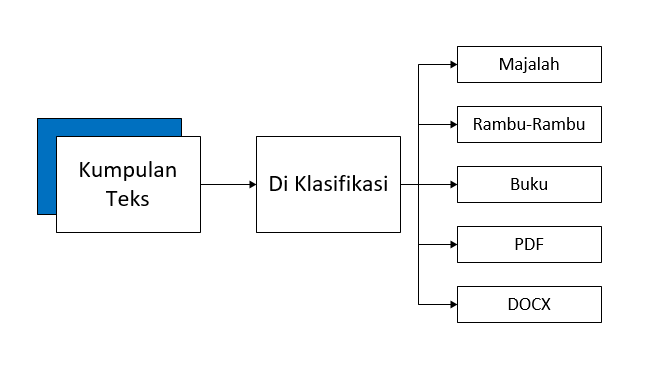
\includegraphics[width=1\textwidth]
      {figures/cokro/c55}}
      \caption{Ilustrasi clasifikasi Teks}
      \label{c55}
      \end{figure}

\begin{figure}
      \centerline{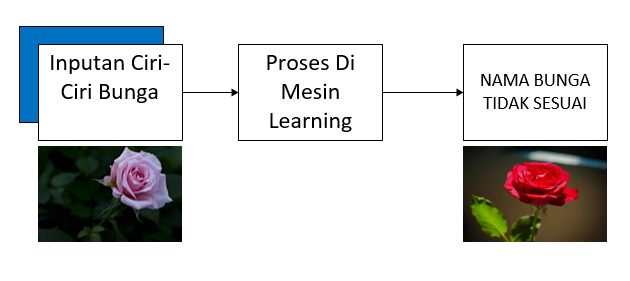
\includegraphics[width=1\textwidth]
      {figures/cokro/c56}}
      \caption{Ilustrasi Bunga Tidak bisa dibaca di Mesin Learning}
      \label{c56}
      \end{figure}

\begin{figure}
      \centerline{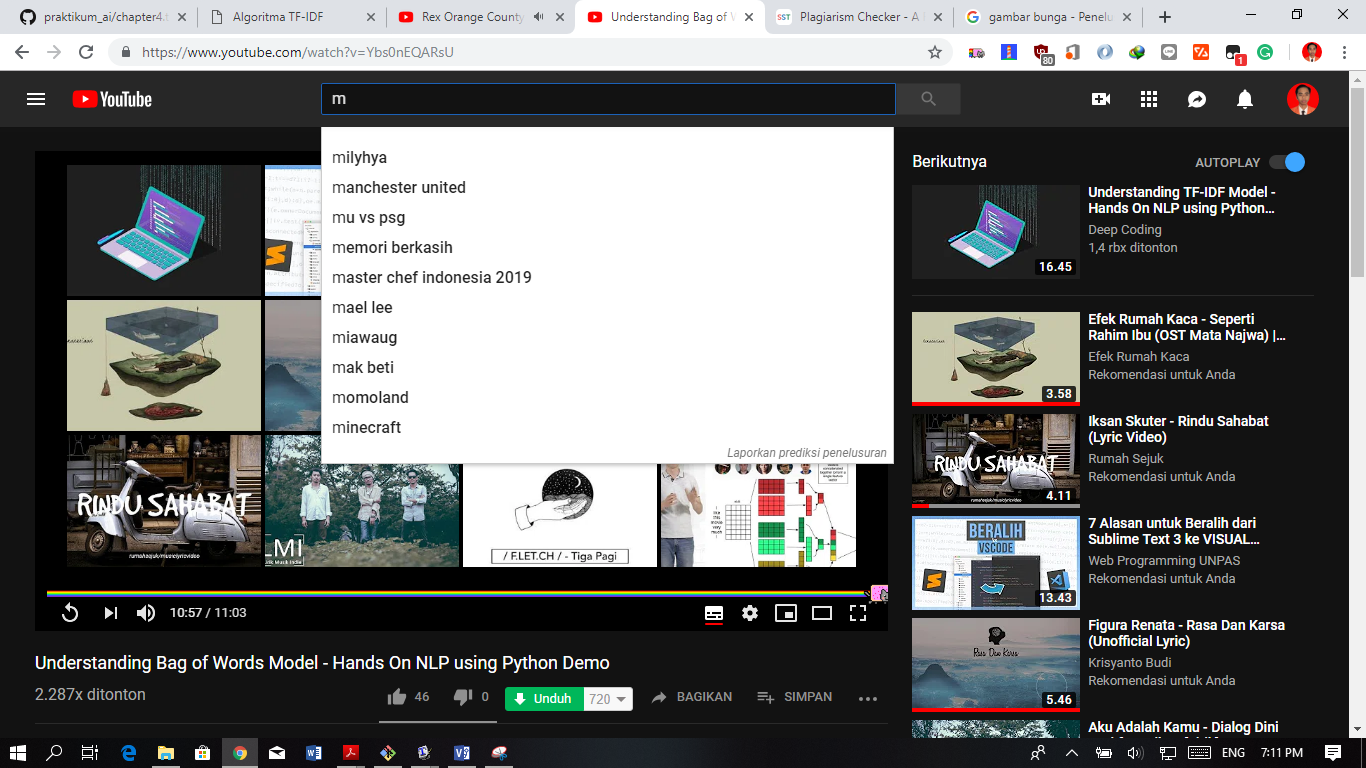
\includegraphics[width=1\textwidth]
      {figures/cokro/c57}}
      \caption{contoh hasil pembelajaran text di youtube}
      \label{c57}
      \end{figure}

\begin{figure}
      \centerline{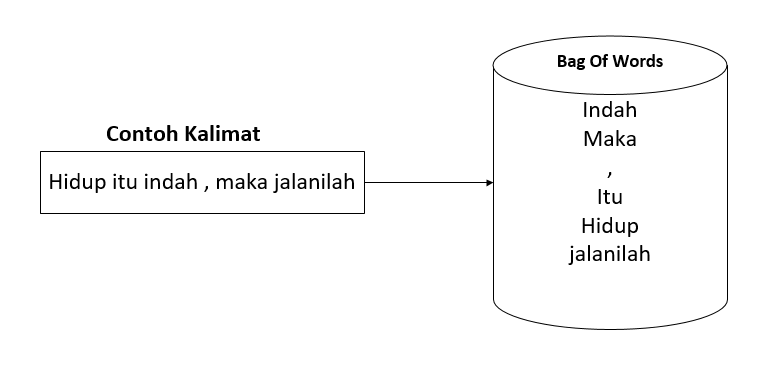
\includegraphics[width=1\textwidth]
      {figures/cokro/c58}}
      \caption{Ilustrasi bag of words}
      \label{c58}
      \end{figure}

\begin{figure}
      \centerline{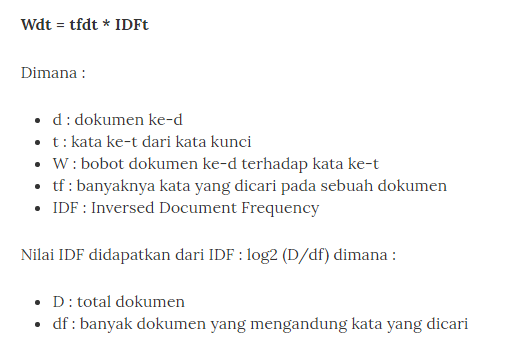
\includegraphics[width=1\textwidth]
      {figures/cokro/c59}}
      \caption{Rumus  TF-IDF}
      \label{c59}
      \end{figure}

\begin{figure}
      \centerline{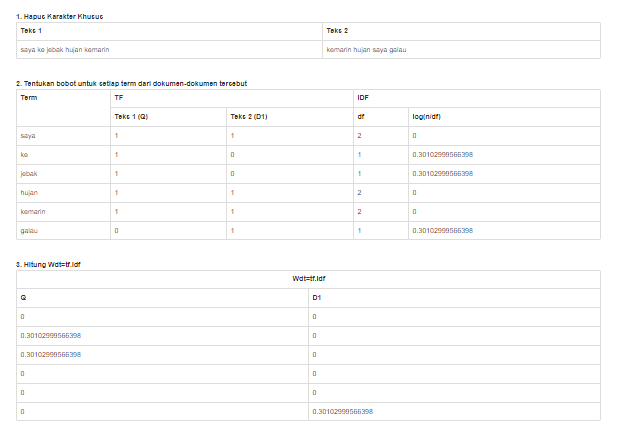
\includegraphics[width=1\textwidth]
      {figures/cokro/c60}}
      \caption{Hasil Perhitungan TF-IDF}
      \label{c60}
      \end{figure}

\begin{figure}
      \centerline{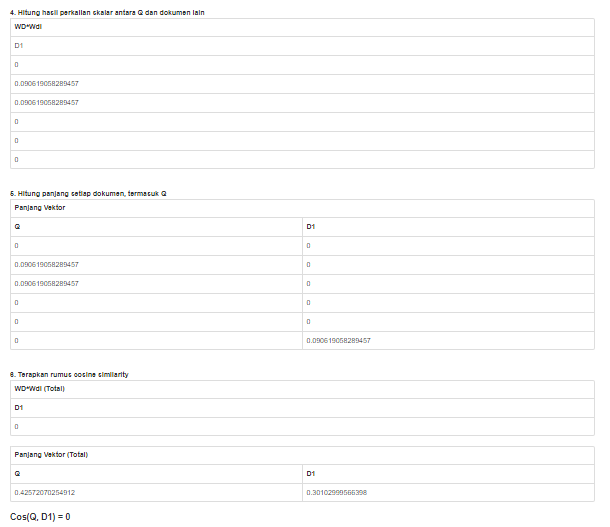
\includegraphics[width=1\textwidth]
      {figures/cokro/c61}}
      \caption{Hasil Perhitungan  TF-IDF}
      \label{c61}
      \end{figure}

\begin{figure}
      \centerline{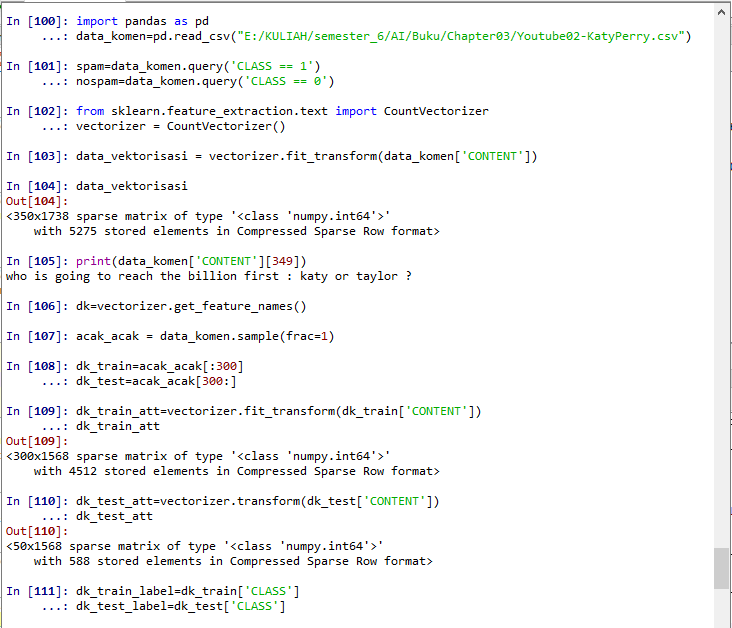
\includegraphics[width=1\textwidth]
      {figures/cokro/c62}}
      \caption{Hasil running data vektorisasi}
      \label{c62}
      \end{figure}

\begin{figure}
      \centerline{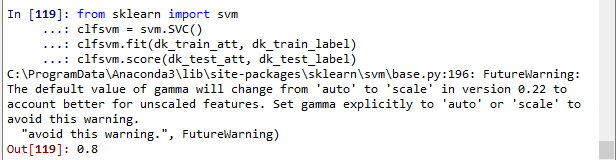
\includegraphics[width=1\textwidth]
      {figures/cokro/c63}}
      \caption{Hasil running klasifikasi svm menggunakan data vektorisasi}
      \label{c63}
      \end{figure}

\begin{figure}
      \centerline{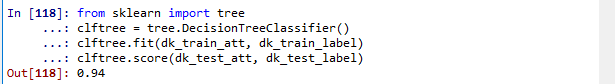
\includegraphics[width=1\textwidth]
      {figures/cokro/c64}}
      \caption{Hasil running klasifikasi decision treei}
      \label{c64}
      \end{figure}

\begin{figure}
      \centerline{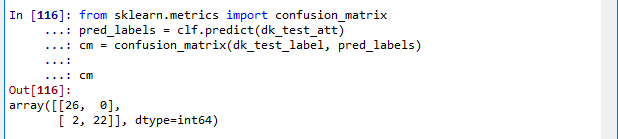
\includegraphics[width=1\textwidth]
      {figures/cokro/c65}}
      \caption{Hasil running cnfusion matrix}
      \label{c65}
      \end{figure}

\begin{figure}
      \centerline{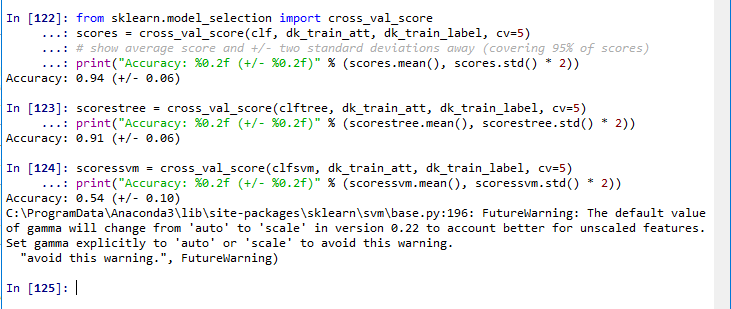
\includegraphics[width=1\textwidth]
      {figures/cokro/c66}}
      \caption{Hasil Cross Validationi}
      \label{c66}
      \end{figure}

\begin{figure}
      \centerline{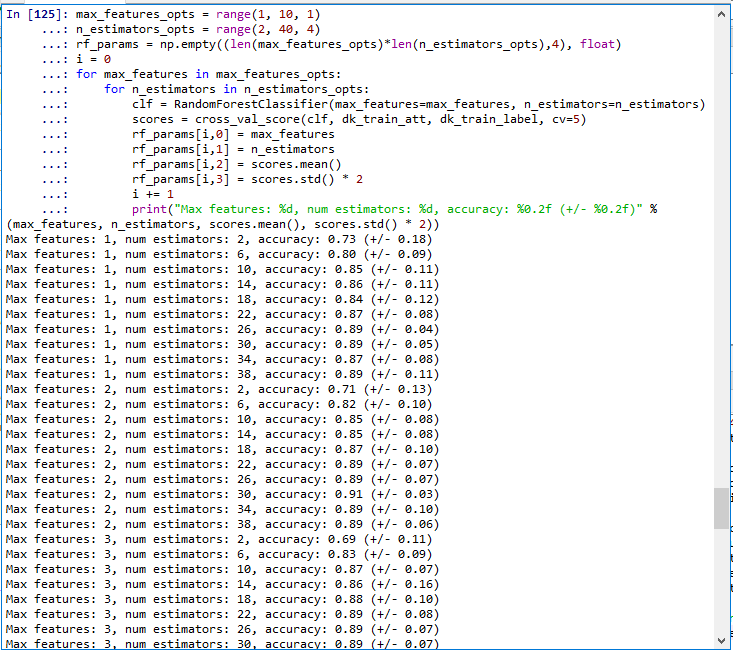
\includegraphics[width=1\textwidth]
      {figures/cokro/c67}}
      \caption{pengulangan Isi Grafik}
      \label{c67}
      \end{figure}

\begin{figure}
      \centerline{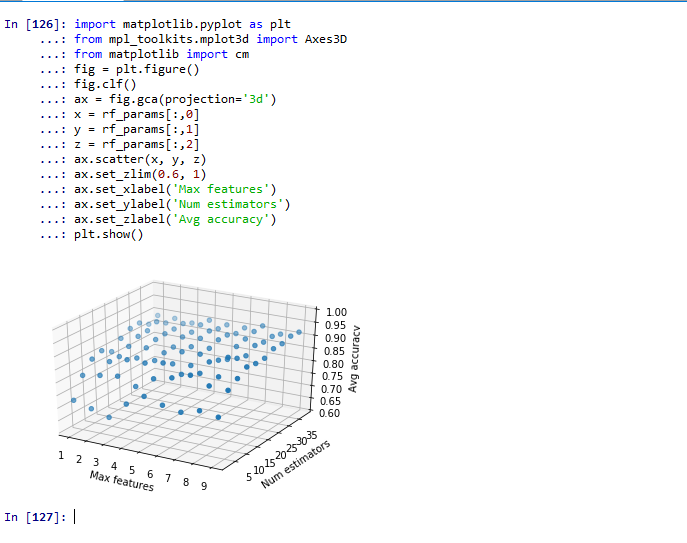
\includegraphics[width=1\textwidth]
      {figures/cokro/c68}}
      \caption{Grafik 3D}
      \label{c68}
      \end{figure}

\begin{figure}
      \centerline{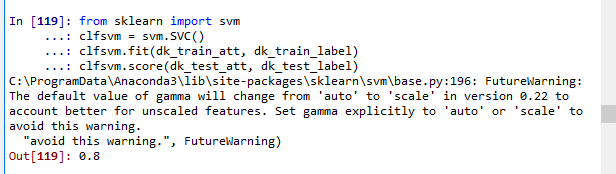
\includegraphics[width=1\textwidth]
      {figures/cokro/c69}}
      \caption{Gambar Warning}
      \label{c69}
      \end{figure}

\begin{figure}
      \centerline{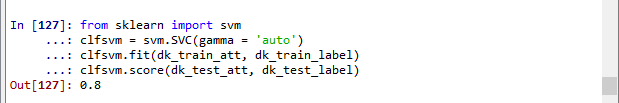
\includegraphics[width=1\textwidth]
      {figures/cokro/c70}}
      \caption{Hasil penanganan Error}
      \label{c70}
      \end{figure}


\section{Fathi Rabbani / 1164074}
\subsection{Teori}
\begin{enumerate}
\item Klasifikasi Teks
\subitem klasifikasi teks adalah sebuah cara dalam memilah data teks berdasarkan beberapa parameter tertentu dengan data yang bersifat dokumen ataupun teks yang memiliki kumpulan - kumpulan teks didalamnya, serta teks itu sendiri merupakan sebuah data yang bisa dibaca oleh manusia atau bisa disebut juga dengan tipe data karakter atau string yang mudah untuk diolah seperti pada buku, majalah, koran, jurnal dan lainya. untuk ilustrasi dari klasifikasi teks bisa dilihat pada gambar \ref{coba1}
\begin{figure}[!htbp]
	\centering
	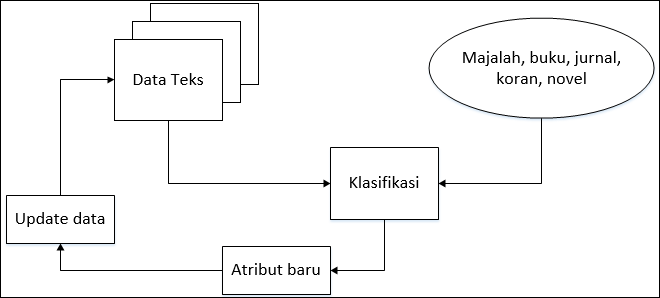
\includegraphics[width=1\textwidth]{figures/fathi/chapter4/hari1/1}
	\caption{Klasifikasi Teks}
	\label{coba1}
\end{figure}

\item Mengapa Klasifikasi Bunga tidak dapat menggunakan Machine Learning
\subitem klasifikasi menggunakan tipe data yang dimana attributenya memiliki nilai data berupa vektor dengan perbandingan masing - masing data yang dimiliki memiliki sedikit perbedaan, sehingga program atau sistem tidak dapat membedakan dengan tepat antara gambar 1 dan gambar 2 dikarenakan memiliki perbedaan yang hampir tidak dapat dilihat pada beberapa contoh gambar. untuk ilustrasi dapat dilihat pada gambar \ref{coba2}
\begin{figure}[!htbp]
	\centering
	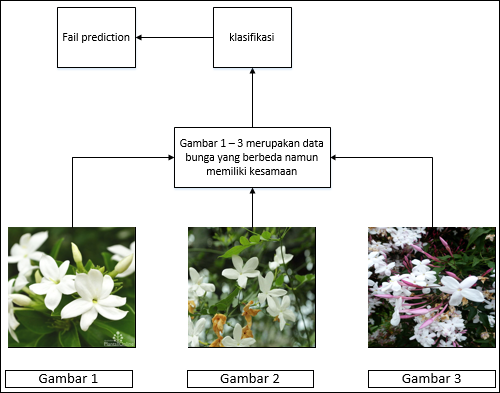
\includegraphics[width=1\textwidth]{figures/fathi/chapter4/hari1/2}
	\caption{Klasifikasi Bunga}
	\label{coba2}
\end{figure}

\item Teknik Pembelajaran Youtube pada Teks
\subitem Youtube merupakan platform untuk berbagi pengalaman video para penggunanya, dan yotube menggunakan machine learning dengan membaca data yang penggunanya inputkan disebut juga temporary data, yang menyimpan data pencarian para penggunanya dengan membuatkan kolom klasifikasinya seperti pada gambar \ref{coba3}, dimana data pencarian saya memliki 6 data dengan jumlah atribut yang masuk adalah 15.
\begin{figure}[!htbp]
	\centering
	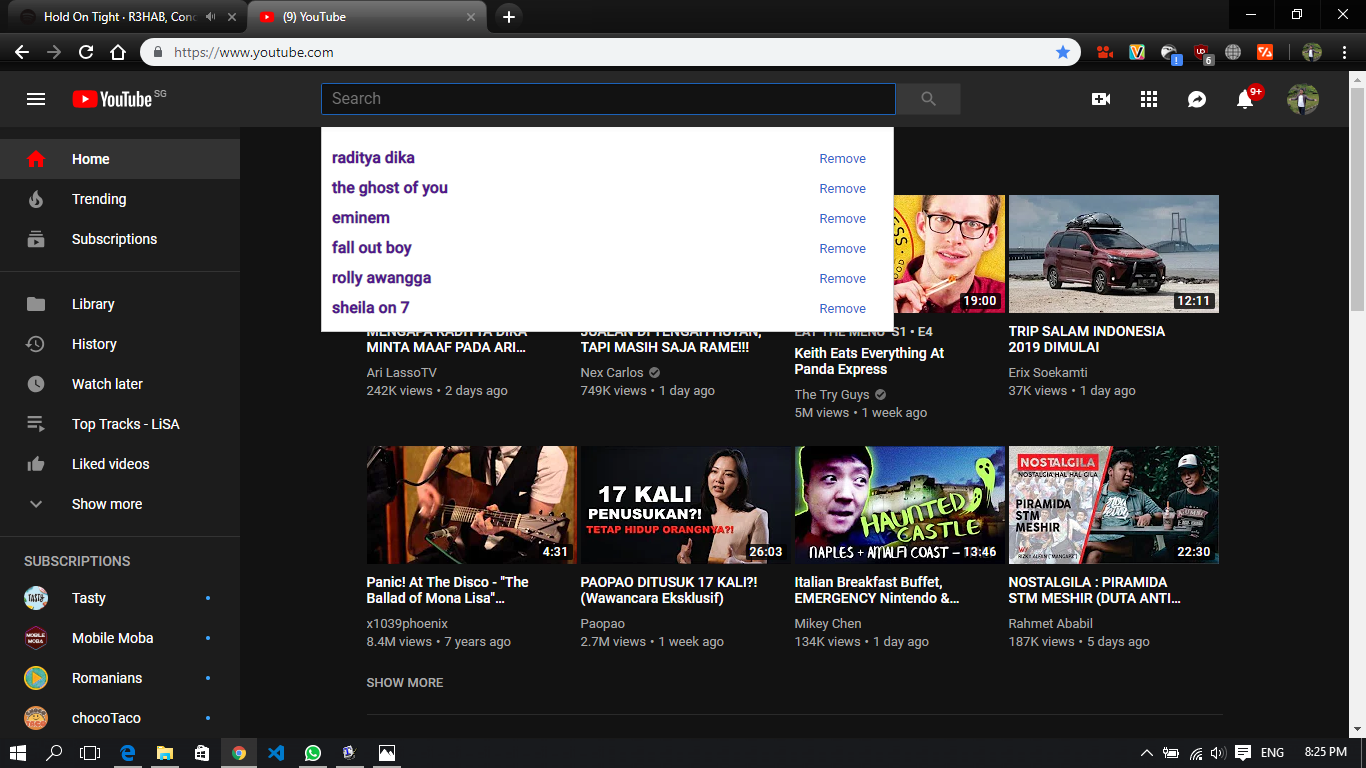
\includegraphics[width=1\textwidth]{figures/fathi/chapter4/hari1/3}
	\caption{Data Youtube}
	\label{coba3}
\end{figure}

\item Vektorisasi Data
\subitem vektor adalah tipe data yang digunakan untuk mempelajari data gambar agar mudah untuk diproses serta lebih sederhana dalam hasil yang dikeluarkan, dan data yang telah divektorisasi terpecah - pecah menjadi beberapa atribut agar mudah untuk diproses.

\item Bag of Words
\subitem kumpulan data teks yang diproses dan dibuatkan atribut barunya jika data yang dimiliki sudah tersedia, pada gambar \ref{coba4}, menjelaskan jika data yang sama tidak akan diproses menjadi atribut baru sehingga data tersebut sudah disimpan dan akan memproses data baru yang belum dimiliki.
\begin{figure}[!htbp]
	\centering
	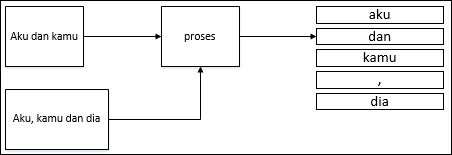
\includegraphics[width=1\textwidth]{figures/fathi/chapter4/hari1/4}
	\caption{Bags of Word}
	\label{coba4}
\end{figure}

\item TF-IDF
\subitem merupakan sebuah metode dalam sebuah perhitungan untuk menghitung bobot dari setiap kata - kata yang sering muncul dalam sebuah kalimat. metode ini sendiri menghitung data nilai dari TF(term of frequency) dan data IDF(inverse document frequency) yang dijadikan sebagai data yang dapat diproses, seperti berikut ini :
\begin{itemize}
\item proses pertama adalah dengan membuat data yang akan diolah seperti pada data 
\begin{verbatim}
–  gold
–  silver
–  truck

Untuk koleksi dokumennya terdapat:

dokumen 1 (d1) = Shipment of gold damaged in a fire
dokumen 2 (d2) = Delivery of silver arrived in a silver truck
dokumen 3 (d3) = Shipment of gold arrived in a truck

Jadi total jumlah dokumen adalah koleksi dokumen (D) = 3
\end{verbatim}

\item proses kedua adalah menggabungkan ke 3 data tersebut dengan menghilangkan nilai yang di ulang (term of frequency)-nya dan hasilnya adalah seperti pada 
\begin{verbatim}
– ship – gold – damage – fire – deliver – silver – arrive – truck
\end{verbatim}

\item kedua proses tersebut dinamakan preprocessing text, dan berikut ini adalah formula yang digunakan untuk menghitung nilai pada bobot data d2 pada
\begin{verbatim}
Wij = TFij x log(D/DFj) + 1
Wij = 2 x (log(3/1) + 1)
Wij = 2 x (0.477 + 1)
Wij = 2.954
\end{verbatim}

\item dengan nilai yang dimiliki seperti itu maka untuk hasilnya adalah seperti pada gambar \ref{coba5}
\begin{figure}[!htbp]
	\centering
	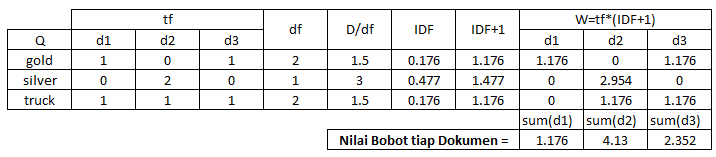
\includegraphics[width=1\textwidth]{figures/fathi/chapter4/hari1/5}
	\caption{TF-IDF}
	\label{coba5}
\end{figure}
\end{itemize}
\end{enumerate}